\documentclass[../main.tex]{subfiles}
\begin{document}
\subsection{Гистограммы и графики плотности распределения}
	\begin{figure}[H]
		\centering
		\begin{tabular}{ccc}
			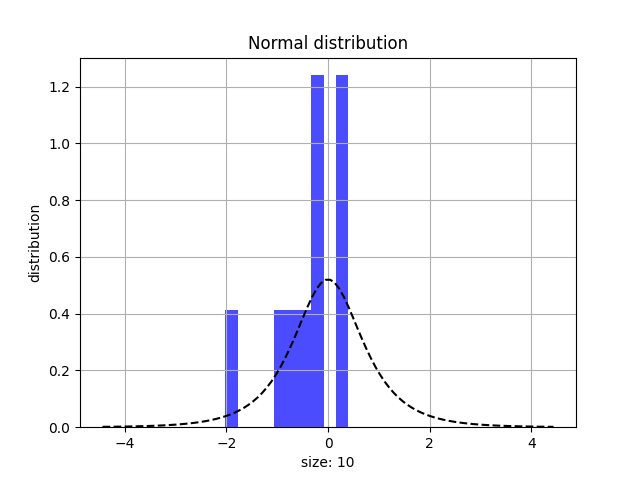
\includegraphics[width=55mm, height  =0.25\textheight]{figures/norm_10.png}
			&
			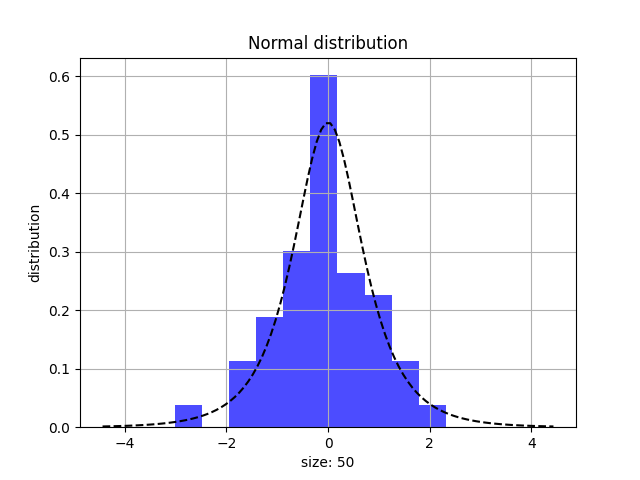
\includegraphics[width=55mm, height  =0.25\textheight]{figures/norm_50.png}
			&
			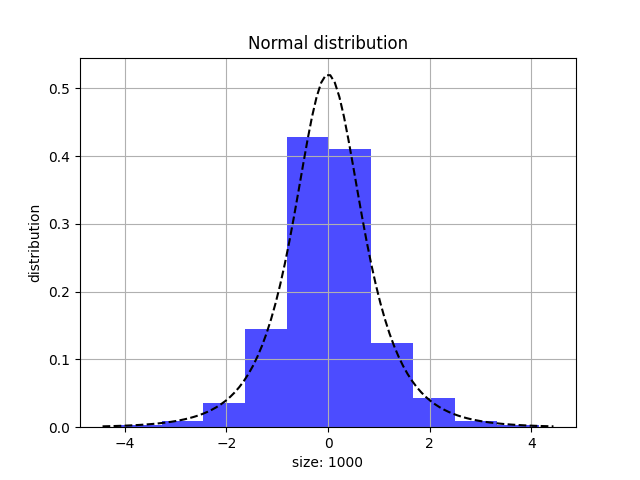
\includegraphics[width=55mm, height=0.25\textheight]{figures/norm_1000.png}
		\end{tabular}
		\caption{Нормальное распределение} 
		\label{fig:normal}
	\end{figure}
	
	\begin{figure}[H]
		\centering
		\begin{tabular}{ccc}
			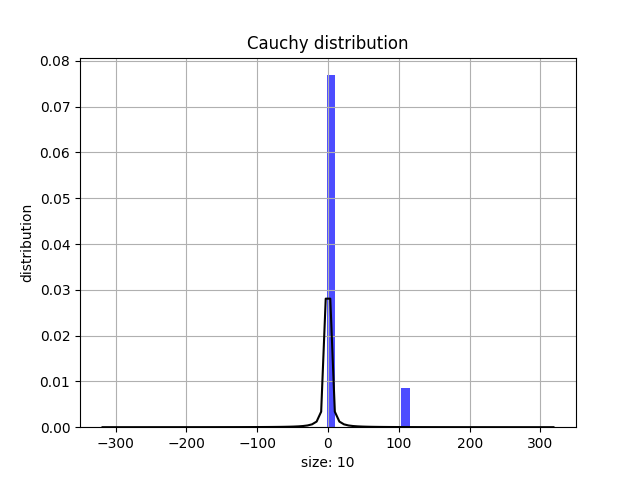
\includegraphics[width=55mm, height =0.25\textheight]{figures/cauchy_10.png} 
			&
			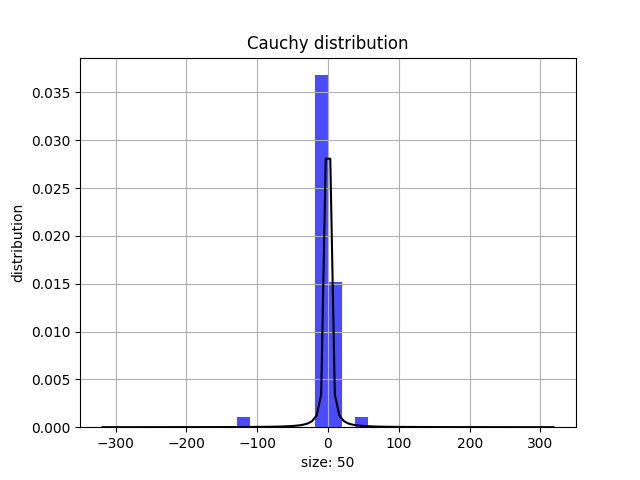
\includegraphics[width=55mm, height =0.25\textheight]{figures/cauchy_50.png}
			&
			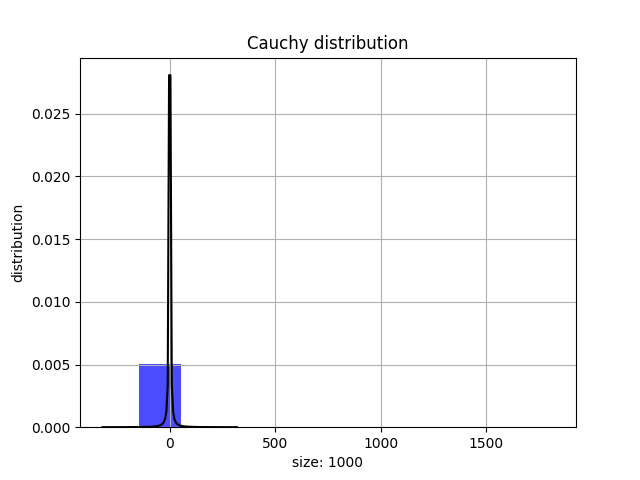
\includegraphics[width=55mm, height =0.25\textheight]{figures/cauchy_1000.png}
		\end{tabular}
		\caption{Распределение Коши} 
		\label{fig:normal}
	\end{figure}
	
	\begin{figure}[H]
		\centering
		\begin{tabular}{ccc}
			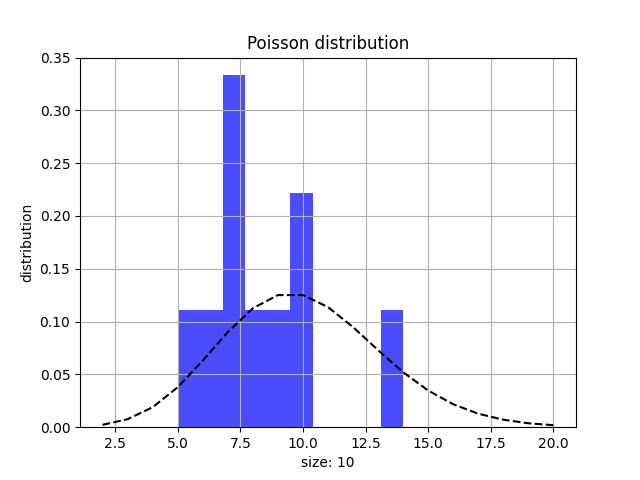
\includegraphics[width=55mm, height =0.25\textheight]{figures/poisson_10.png} 
			&
			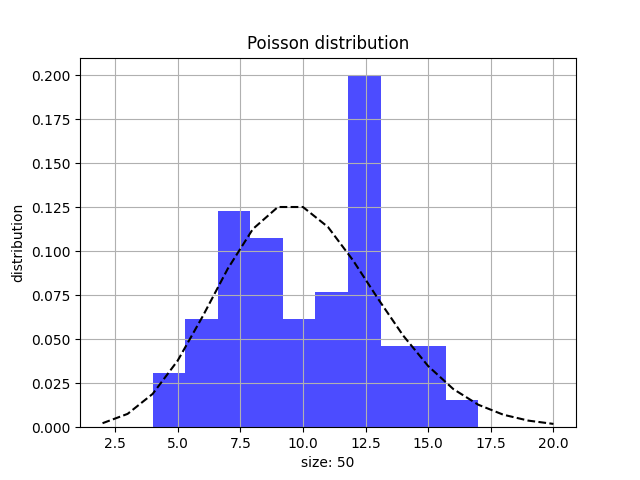
\includegraphics[width=55mm, height =0.25\textheight]{figures/poisson_50.png}
			&
			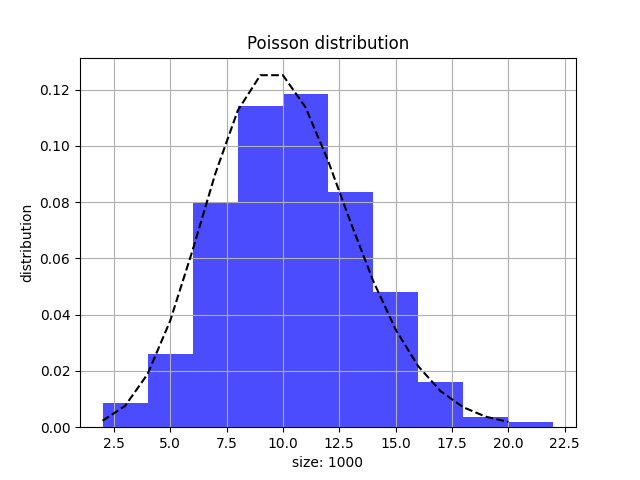
\includegraphics[width=55mm, height =0.25\textheight]{figures/poisson_1000.png}
		\end{tabular}
		\caption{Распределение Пауссона} 
		\label{fig:normal}
	\end{figure}
	
	\begin{figure}[H]
		\centering
		\begin{tabular}{ccc}
			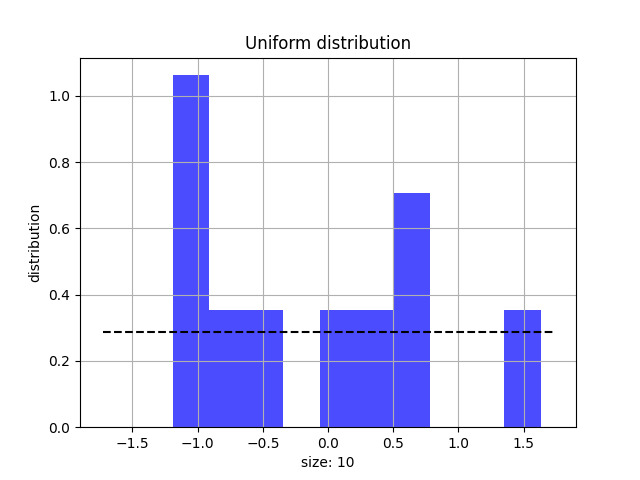
\includegraphics[width=55mm, height =0.25\textheight]{figures/uniform_10.png} 
			&
			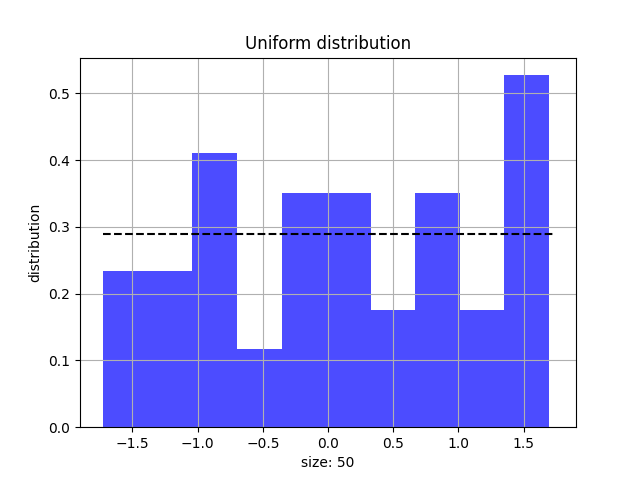
\includegraphics[width=55mm, height =0.25\textheight]{figures/uniform_50.png}
			&
			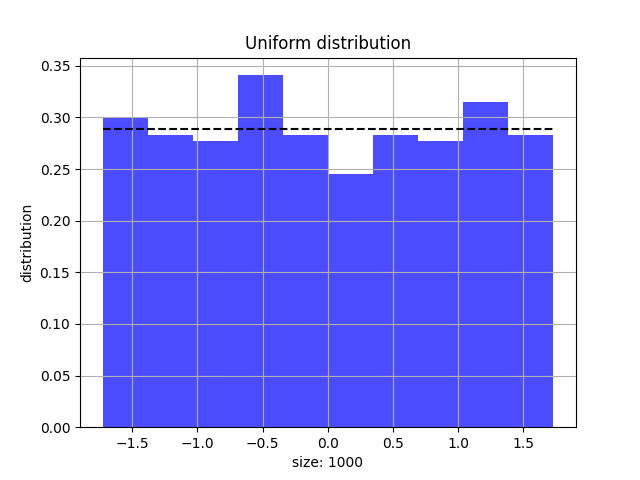
\includegraphics[width=55mm, height =0.25\textheight]{figures/uniform_1000.png}
		\end{tabular}
		\caption{Равномерное распределение} 
		\label{fig:normal}
	\end{figure}
	
	\subsection{Характеристики положения и рассеяния}
	
	\begin{table}[H]
    \centering
    \begin{tabular}{|l||c|c|c|c|c|}
        \hline
        & $\overline{x}$ & $med x$ & $z_R$ & $z_Q$ & $z_{tr}$\\\hline\hline
        n=10 & & & & &\\\hline
        $E(z)$ & -0.00348 & 0.004 & -0.002019 & 0.310749 & 0.272089\\\hline
        $D(z)$ & 0.097069 & 0.136516 & 0.180398 & 0.121412 & 0.113616\\\hline
        E(z) \pm \sqrt{D(z)} & [0.308079; & [0.373481; & [0.422714; & [0.659191; & [0.609159;\\
		&  -0.315039] & -0.365481] & -0.426752] & -0.037693] & -0.064981] \\\hline
		\widehat{E}(z) & 0 & 0 & 0 & 0 & 0\\\hline
        n=100 & & & & &\\\hline
        $E(z)$ & -0.00067 & 0.003322 & 0.000155 & 0.016217 & 0.027022\\\hline
        $D(z)$ & 0.009173 & 0.015399 & 0.094144 & 0.011524 & 0.011703\\\hline
        E(z) \pm \sqrt{D(z)} & [0.095106; & [0.127415; & [0.306984; & [0.123567; & [0.135202;\\
		& -0.096446] & -0.120771] & -0.306674] & -0.091133] & -0.081158] \\\hline
		\widehat{E}(z) & 0 & 0 & 0 & 0 & 0\\\hline
        n=1000 & & & & &\\\hline
        $E(z)$ & -0.000533 & -0.000974 & -0.002506 & 0.001507 & 0.002228\\\hline
        $D(z)$ & 0.001016 & 0.001602 & 0.056853 & 0.001242 & 0.001243\\\hline
        E(z) \pm \sqrt{D(z)} & [0.031342; & [0.039051; & [0.235933; & [0.036749; & [0.037484; \\
		&  -0.032408] & -0.040999] & -0.240945] & -0.033735] & -0.033028] \\\hline
		\widehat{E}(z) & 0.0 & 0.0 & 0 & 0.0 & 0.0\\\hline
    \end{tabular}
    \caption{Нормальное распределение}
    \label{tab:normal}
    \end{table}
    
    \begin{table}[H]
    \centering
    \begin{tabular}{|l||c|c|c|c|c|}
        \hline
        & $\overline{x}$ & $med x$ & $z_R$ & $z_Q$ & $z_{tr}$\\\hline\hline
        n=10 & & & & &\\\hline
        $E(z)$ & 1.467166 & -0.001573 & 7.221644 & 1.206193 & 0.716898\\\hline
        $D(z)$ & 310.55165 & 0.31919 & 7623.471253 & 5.887761 & 1.389557\\\hline
        E(z) \pm \sqrt{D(z)} & [19.089642; & [0.563396; & [94.534136; & [3.632664; & [1.895693; \\
		&  -16.15531] & -0.566542] & -80.090848] & -1.220278] & -0.461897] \\\hline
		\widehat{E}(z) & - & 0 & - & - & -\\\hline
        n=100 & & & & &\\\hline
        $E(z)$ & -0.403601 & -0.00268 & -18.256451 & 0.032517 & 0.039435\\\hline
        $D(z)$ & 207.042142 & 0.02548 & 474814.408027 & 0.051517 & 0.026261\\\hline
        E(z) \pm \sqrt{D(z)} & [13.985358; & [0.156945; & [670.811331; & [0.259491; & [0.201487; \\
		&  -14.792560] & -0.162305] & -707.324233] & -0.194457] & -0.122617] \\\hline
		\widehat{E}(z) & - & 0 & - & 0 & 0\\\hline
        n=1000 & & & & &\\\hline
        $E(z)$ & 1.96279 & 0.000414 & 957.214575 & 0.003529 & 0.003743\\\hline
        $D(z)$ & 2298.90608 & 0.002494 & 572736372.167594 & 0.00509 & 0.002531\\\hline
        E(z) \pm \sqrt{D(z)} & [49.909699; & [0.050354; & [24889.125743; & [0.074873; & [0.054052; \\
		&  -45.984119] & -0.049526] & -22974.696593] & -0.067815] & -0.046566] \\\hline
		\widehat{E}(z) & - & 0.0 & - & 0.0 & 0.0\\\hline
    \end{tabular}
    \caption{Распределение Коши}
    \label{tab:normal}
    \end{table}
	
	\begin{table}[H]
    \centering
    \begin{tabular}{|l||c|c|c|c|c|}
        \hline
        & $\overline{x}$ & $med x$ & $z_R$ & $z_Q$ & $z_{tr}$\\\hline\hline
        n=10 & & & & &\\\hline
        []
[]
[]
[]
        $E(z)$ & 10.0181 & 9.883 & 10.291 & 10.952 & 10.7875\\\hline
        $D(z)$ & 1.034302 & 1.418311 & 1.938319 & 1.407696 & 1.276816\\\hline
        E(z) \pm \sqrt{D(z)} & [11.035106; & [11.073929; & [11.683235; & [12.138464; & [11.917463; \\
		&  9.001094] & 8.692071] & 8.898765] & 9.765536] & 9.657537] \\\hline
		\widehat{E}(z) & 10^{+1}_{-1} & 10^{+1}_{-1} & 10^{+2}_{-2} & 10^{+2}_{-2} & 10^{+2}_{-2}\\\hline
        n=100 & & & & &\\\hline
        $E(z)$ & 9.9964 & 9.844 & 10.9675 & 9.956 & 9.9361\\\hline
        $D(z)$ & 0.099851 & 0.206164 & 1.032194 & 0.167564 & 0.121291\\\hline
        E(z) \pm \sqrt{D(z)} & [10.312392; & [10.298053; & [11.983469; & [10.365346; & [10.284369; \\
		&  9.680408] & 9.389947] & 9.951531] & 9.546654] & 9.587831] \\\hline
		\widehat{E}(z) & 10^{+1}_{-1} & 10^{+1}_{-1} & 10^{+2}_{-2} & 10^{+1}_{-1} & 10^{+1}_{-1}\\\hline
        n=1000 & & & & &\\\hline
        $E(z)$ & 10.001108 & 9.9965 & 11.664 & 9.9965 & 9.867582\\\hline
        $D(z)$ & 0.009773 & 0.003238 & 0.670604 & 0.002238 & 0.01099\\\hline
        E(z) \pm \sqrt{D(z)} & [10.099966; & [10.053403; & [12.482904; &  [10.043808; & [9.972415; \\
		&  9.90225] & 9.939597] & 10.845096] & 9.949192] & 9.762749] \\\hline
		\widehat{E}(z) & 10^{+1}_{-1} & 10^{+1}_{-1} & 10^{+2}_{-2} & 10^{+1}_{-1} & 10^{+1}_{-1}\\\hline
    \end{tabular}
    \caption{Распределение Пуасона}
    \label{tab:normal}
    \end{table}
    
    \begin{table}[H]
    \centering
    \begin{tabular}{|l||c|c|c|c|c|}
        \hline
        & $\overline{x}$ & $med x$ & $z_R$ & $z_Q$ & $z_{tr}$\\\hline\hline
        n=10 & & & & &\\\hline
        $E(z)$ & 0.003982 & -0.000821 & 0.003601 & 0.325005 & 0.32347\\\hline
        $D(z)$ & 0.098091 & 0.227379 & 0.043689 & 0.129782 & 0.153936\\\hline
        E(z) \pm \sqrt{D(z)} & [0.317177; & [0.476022; & [0.21262; & [0.685258; & [0.715817; \\
		&  -0.309213] & -0.477664] & -0.205418] & -0.035248] & -0.068877] \\\hline
		\widehat{E}(z) & 0 & 0 & 0 & 0 & 0\\\hline
        n=100 & & & & &\\\hline
        $E(z)$ & 0.000791 & -0.000383 & 0.000313 & 0.017294 & 0.035598\\\hline
        $D(z)$ & 0.00971 & 0.030358 & 0.000609 & 0.014141 & 0.01957\\\hline
        E(z) \pm \sqrt{D(z)} & [0.099330; & [0.173852; & [0.024991; &  [0.13621; & [0.175491; \\
		& -0.097748] & -0.174618] & -0.024365] & -0.101622] & -0.104295] \\\hline
		\widehat{E}(z) & 0 & 0 & 0.0 & 0 & 0\\\hline
        n=1000 & & & & &\\\hline
        $E(z)$ & 0.001151 & 0.000858 & -6e-05 & 0.003018 & 0.004825\\\hline
        $D(z)$ & 0.00099 & 0.003027 & 7e-06 & 0.001456 & 0.001995\\\hline
        E(z) \pm \sqrt{D(z)} & [0.032615; & [0.055876; & [0.002586; &  [0.041176; & [0.04949;\\
		& -0.030313] & -0.05416] & -0.002706] & -0.03514] & -0.03984] \\\hline
		\widehat{E}(z) & 0.0 & 0.0 & 0.00 & 0.0 & 0.0\\\hline
    \end{tabular}
    \caption{Равномерное распределение}
    \label{tab:normal}
    \end{table}
	
	\subsection{Боксплот Тьюки}
	
	\begin{figure}[H]
        \centering
        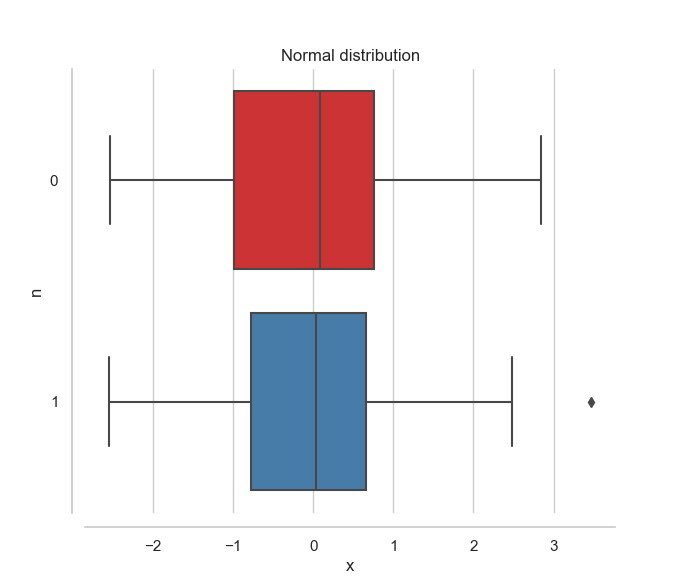
\includegraphics[scale=0.8]{figures/NormalBoxplot.png}
        \caption{Нормальное распределение}
        \label{fig:normal}
    \end{figure}
    
    \begin{figure}[H]
        \centering
        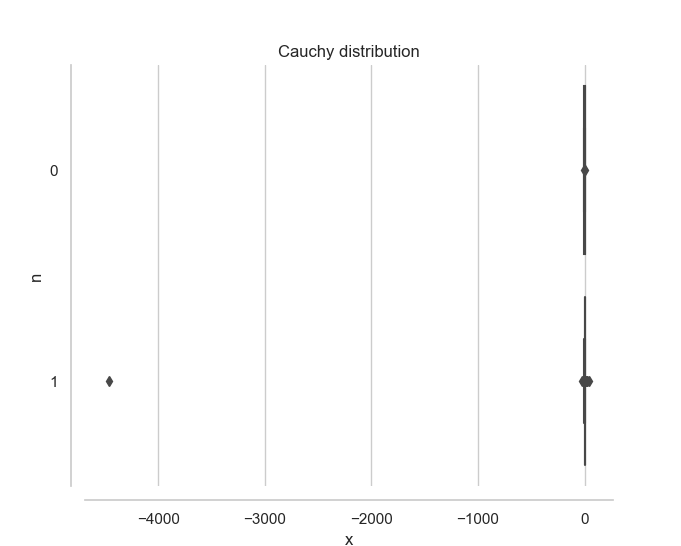
\includegraphics[scale=0.8]{figures/CauchyBoxplot.png}
        \caption{Распределение Коши}
        \label{fig:normal}
    \end{figure}
    
    \begin{figure}[H]
        \centering
        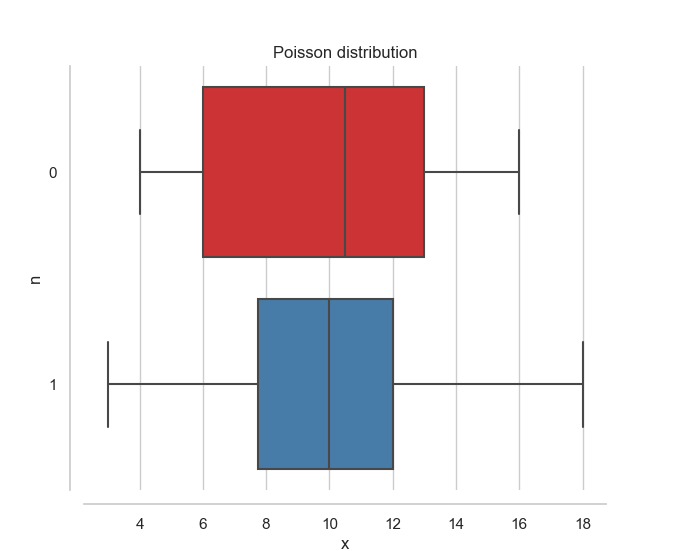
\includegraphics[scale=0.8]{figures/PoissonBoxplot.png}
        \caption{Распределение Пуассона}
        \label{fig:normal}
    \end{figure}
    
    \begin{figure}[H]
        \centering
        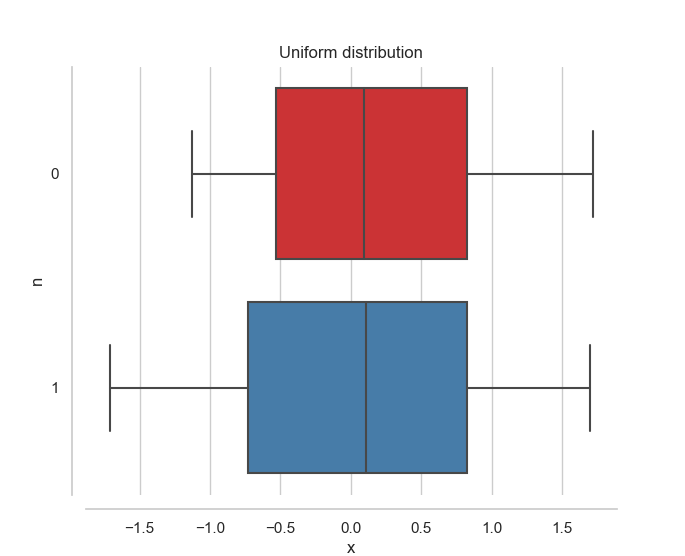
\includegraphics[scale=0.8]{figures/UniformBoxplot.png}
        \caption{Равномерное распределение}
        \label{fig:normal}
    \end{figure}
    
    \subsection{Доля выбросов}
    \begin{table}[H]
	\centering
	\begin{tabular}{|l|c|c|}
		\hline
		Выборка & Доля выбросов	\\\hline
		\hline
		Normal n = 20 & 0.02605 \\\hline
		Normal n = 100 & 0.01043 \\\hline
		Cauchy n = 20 & 0.15155 \\\hline
		Cauchy n = 100 & 0.15624 \\\hline
		Poisson n = 20 & 0.02315 \\\hline
		Poisson n = 100 & 0.01051 \\\hline
		Uniform n = 20 & 0.00195\\\hline
		Uniform n = 100 & 0 \\\hline
	\end{tabular}
	\caption{Практическая доля выбросов}
    \end{table}
    
    \subsection{Теоретическая вероятность выбросов}
    
    \begin{table}[H]
	\centering
	\begin{tabular}{|l|c|c|c|c|c|}
		\hline
		Распределение & $Q_1^T$	& $Q_3^T$ & $X_1^T$ & $X_2^T$ & $P_B^T$\\\hline
		\hline
		Нормальное & -0.674 & 0.674 & -2.698 &  2.698 & 0.007\\\hline
		Коши & -1 & 1 & -4 & 4 & 0.156\\\hline
		Пуассона & 8 & 12 & 2 & 18 & 0.008\\\hline
		Равномерное & -0.866 & 0.866 & -3.464 & 3.464 & 0\\\hline
	\end{tabular}
	\caption{Теоретическая вероятность выбросов}
    \end{table}
    
    \subsection{Эмпирическая функция распределения}
    
    \begin{figure}[H]
        \centering
        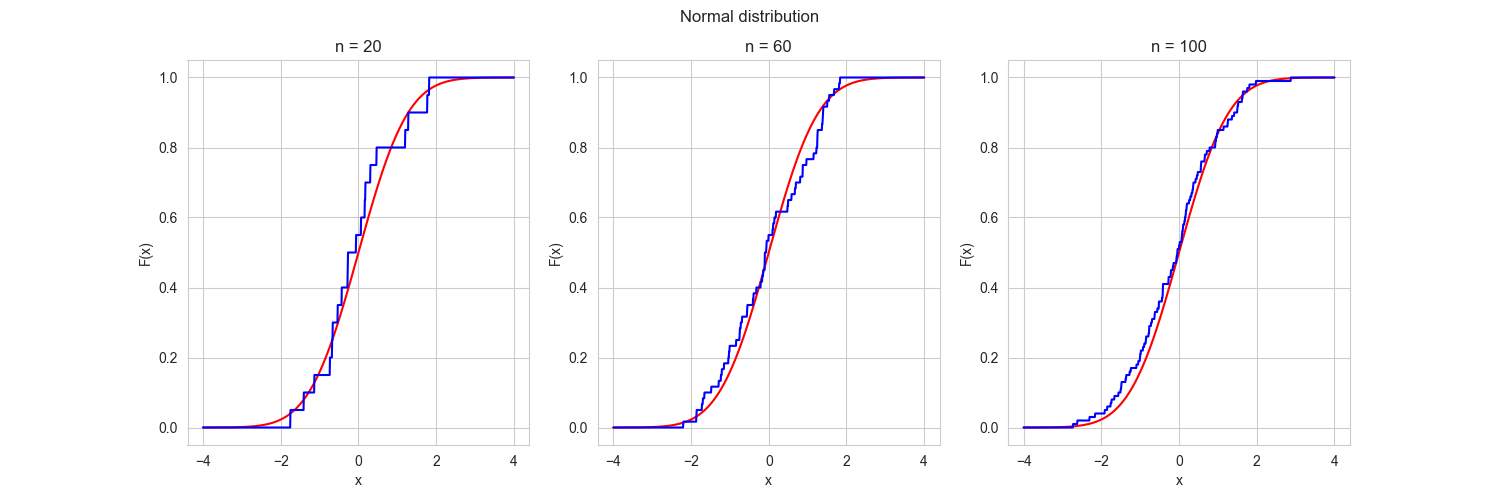
\includegraphics[scale=0.5]{figures/NormalEmpirical.png}
        \caption{Нормальное распределение}
        \label{fig:normal}
    \end{figure}
    
    \begin{figure}[H]
        \centering
        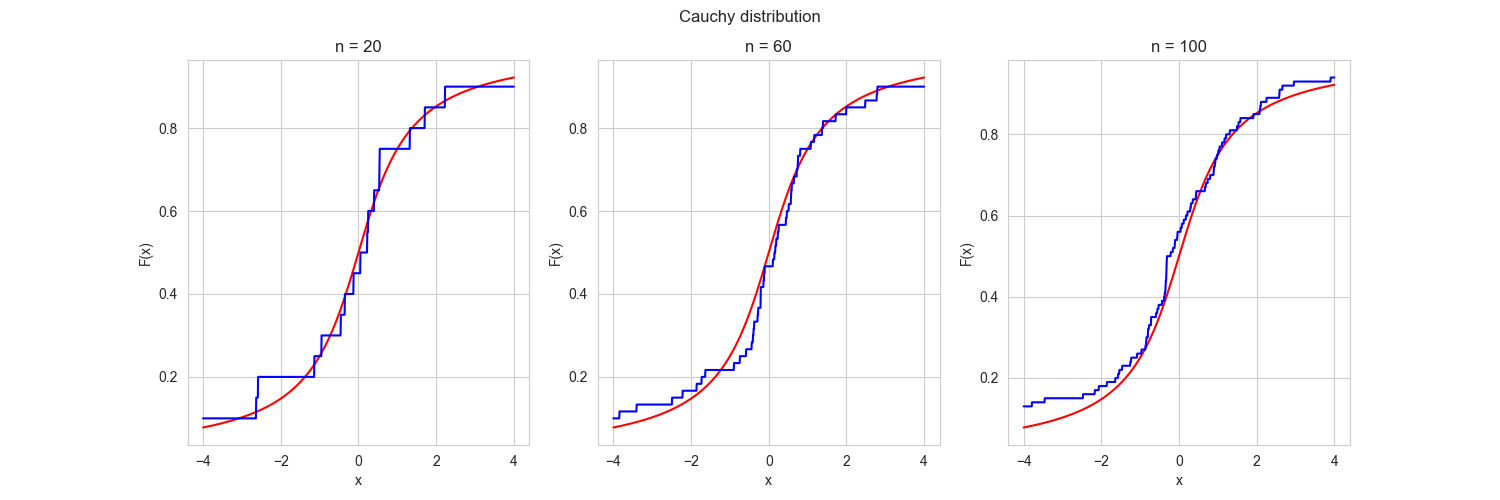
\includegraphics[scale=0.5]{figures/CauchyEmpirical.png}
        \caption{Распределение Коши}
        \label{fig:normal}
    \end{figure}
    
    \begin{figure}[H]
        \centering
        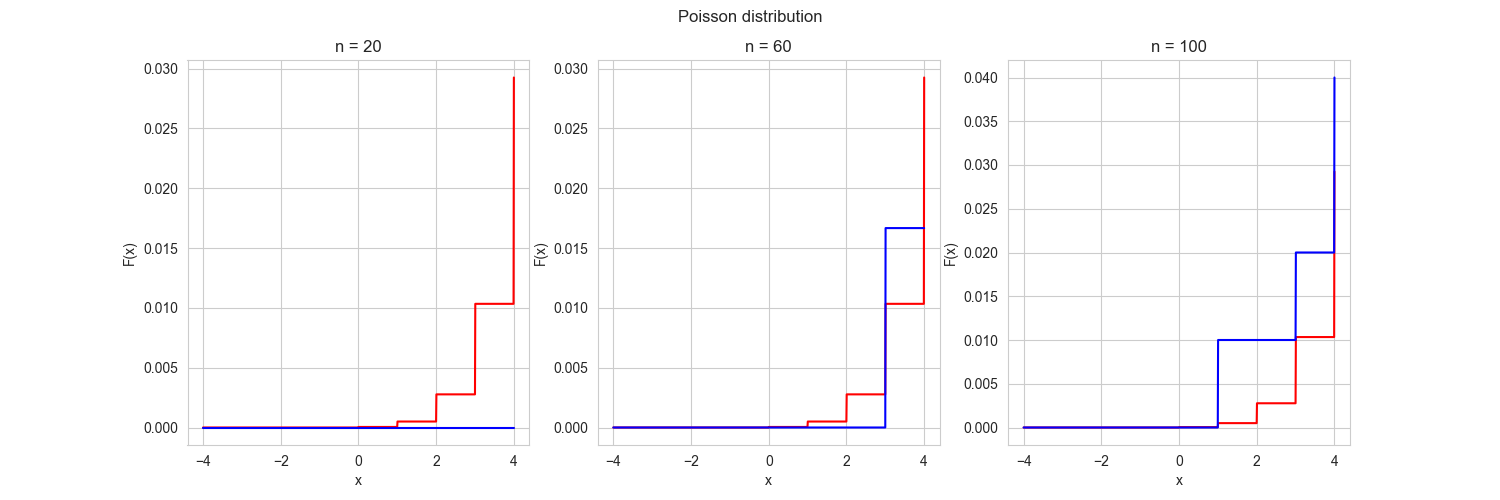
\includegraphics[scale=0.5]{figures/PoissonEmpirical.png}
        \caption{Распределение Пуассона}
        \label{fig:normal}
    \end{figure}
    
    \begin{figure}[H]
        \centering
        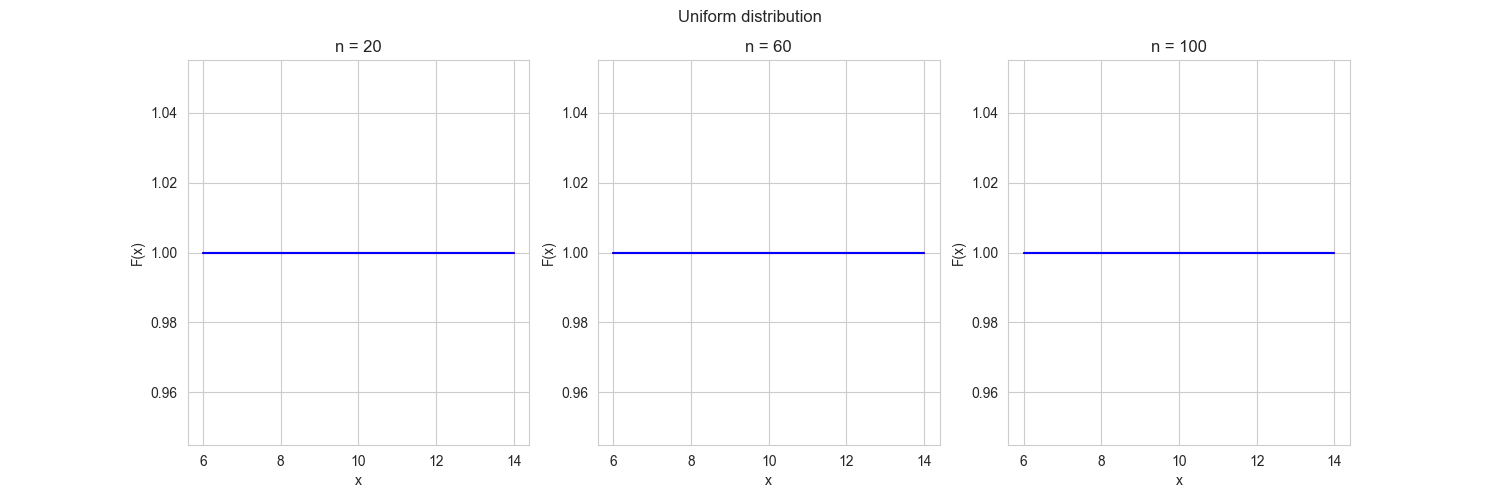
\includegraphics[scale=0.5]{figures/UniformEmpirical.png}
        \caption{Равномерное распределение}
        \label{fig:normal}
    \end{figure}
    
    \subsection{Ядерные оценки плотности распределения}
    
    \begin{figure}[H]
        \centering
        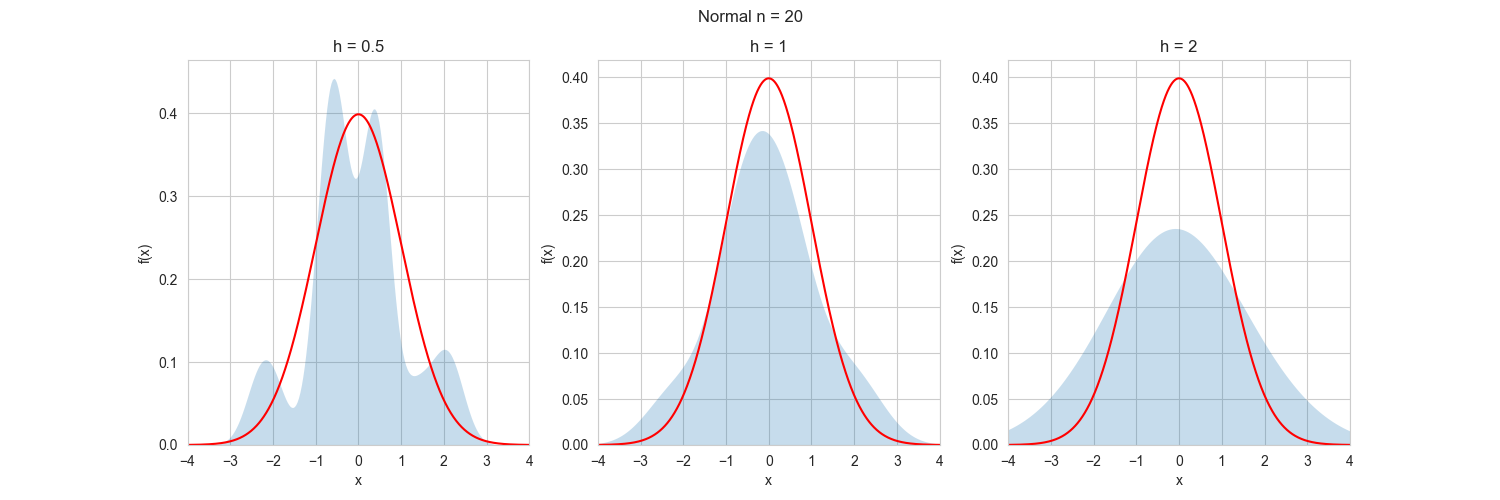
\includegraphics[scale=0.5]{figures/NormalNuclear20.png}
        \caption{Нормальное распределение, n = 20}
        \label{fig:normal}
    \end{figure}
    
    \begin{figure}[H]
        \centering
        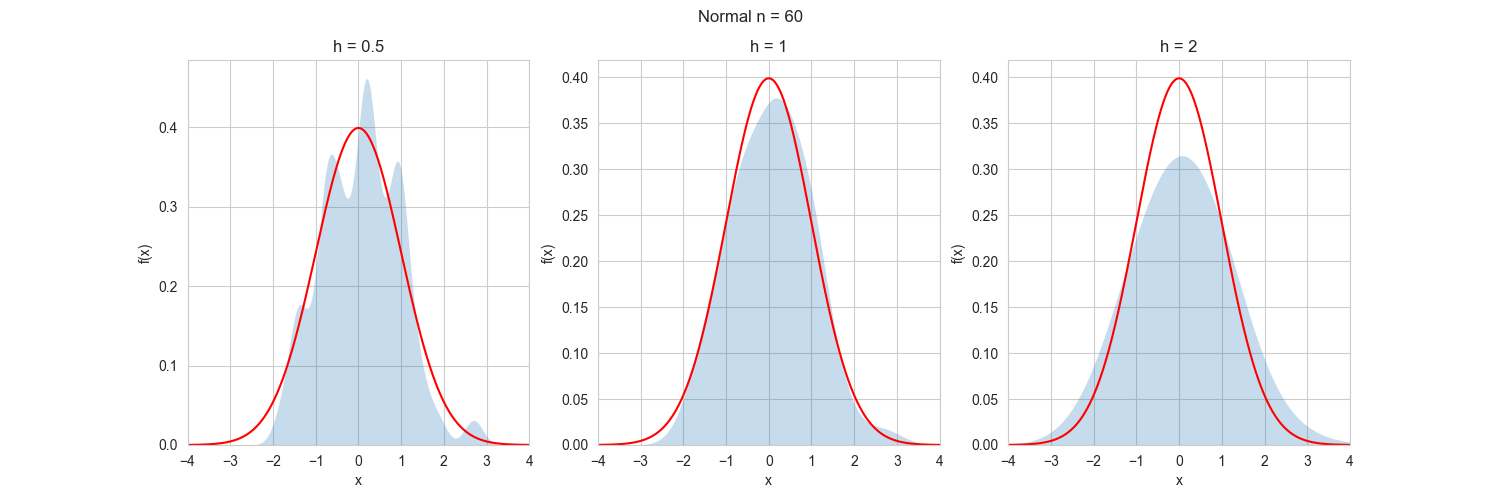
\includegraphics[scale=0.5]{figures/NormalNuclear60.png}
        \caption{Нормальное распределение, n = 60}
        \label{fig:normal}
    \end{figure}
    
    \begin{figure}[H]
        \centering
        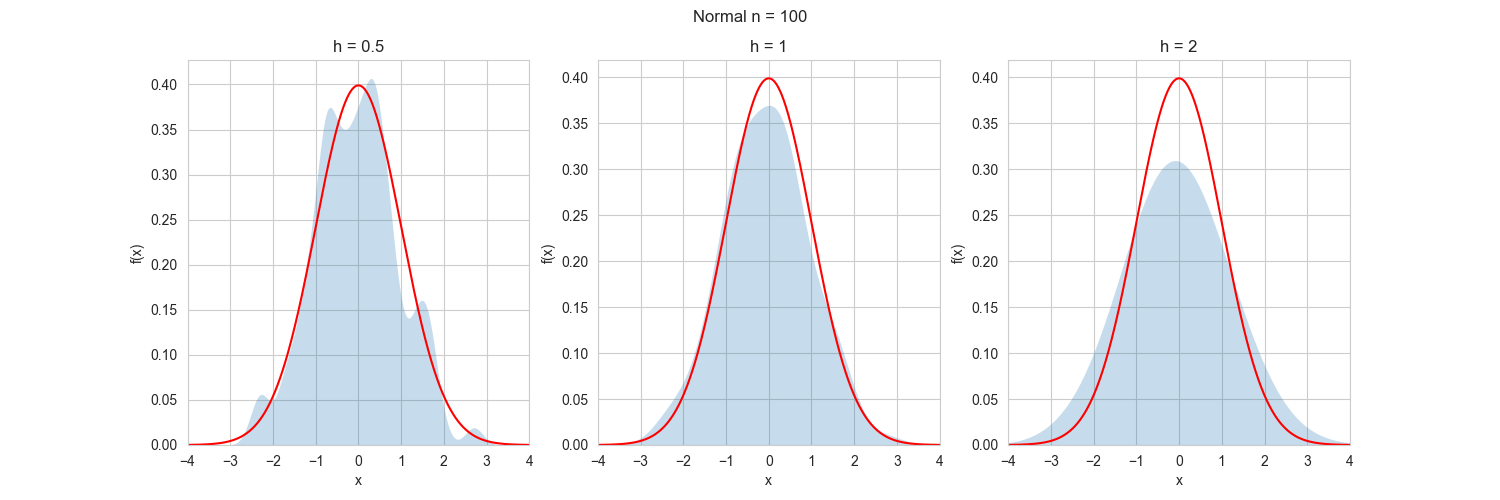
\includegraphics[scale=0.5]{figures/NormalNuclear100.png}
        \caption{Нормальное распределение, n = 100}
        \label{fig:normal}
    \end{figure}
    
    \begin{figure}[H]
        \centering
        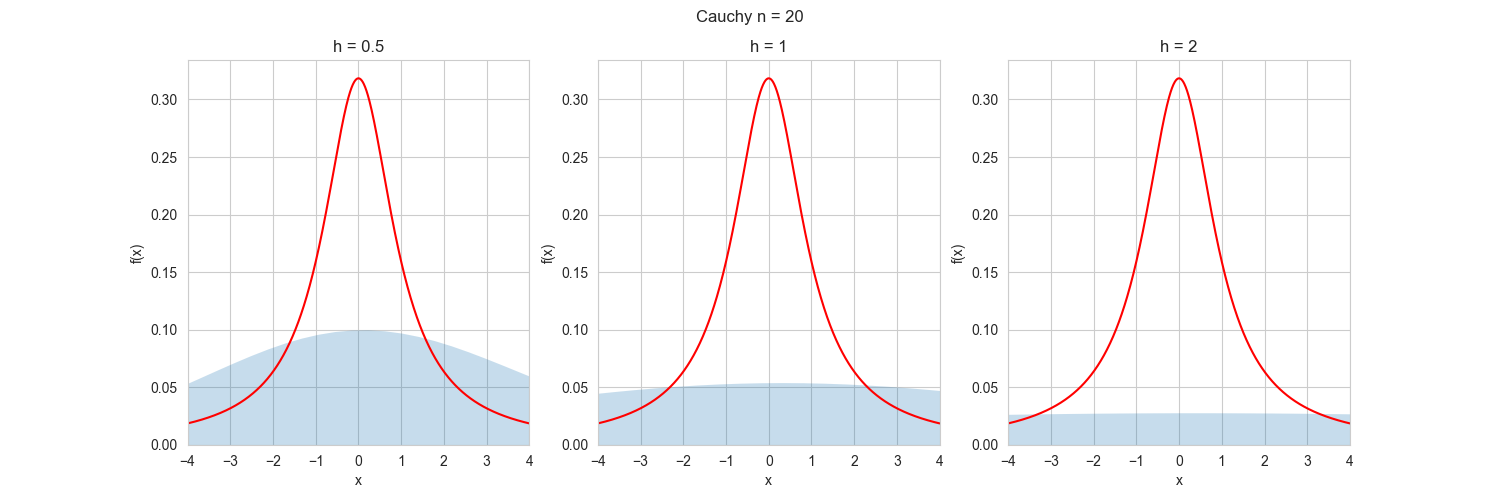
\includegraphics[scale=0.5]{figures/CauchyNuclear20.png}
        \caption{Распределение Коши, n = 20}
        \label{fig:normal}
    \end{figure}
    
    \begin{figure}[H]
        \centering
        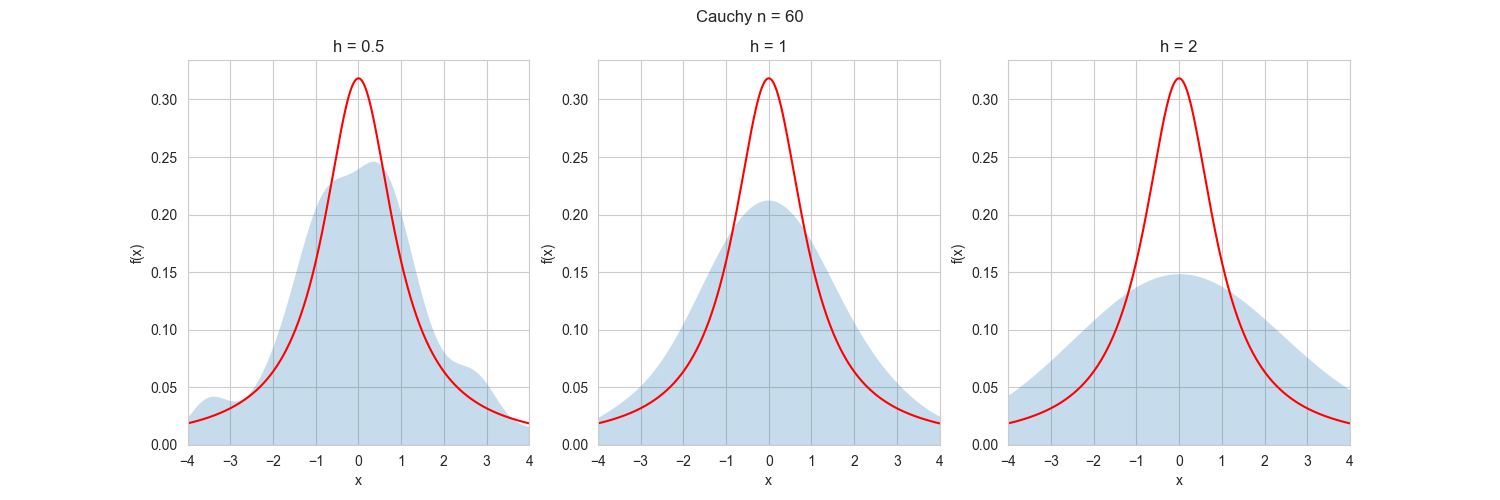
\includegraphics[scale=0.5]{figures/CauchyNuclear60.png}
        \caption{Распределение Коши, n = 60}
        \label{fig:normal}
    \end{figure}
    
    \begin{figure}[H]
        \centering
        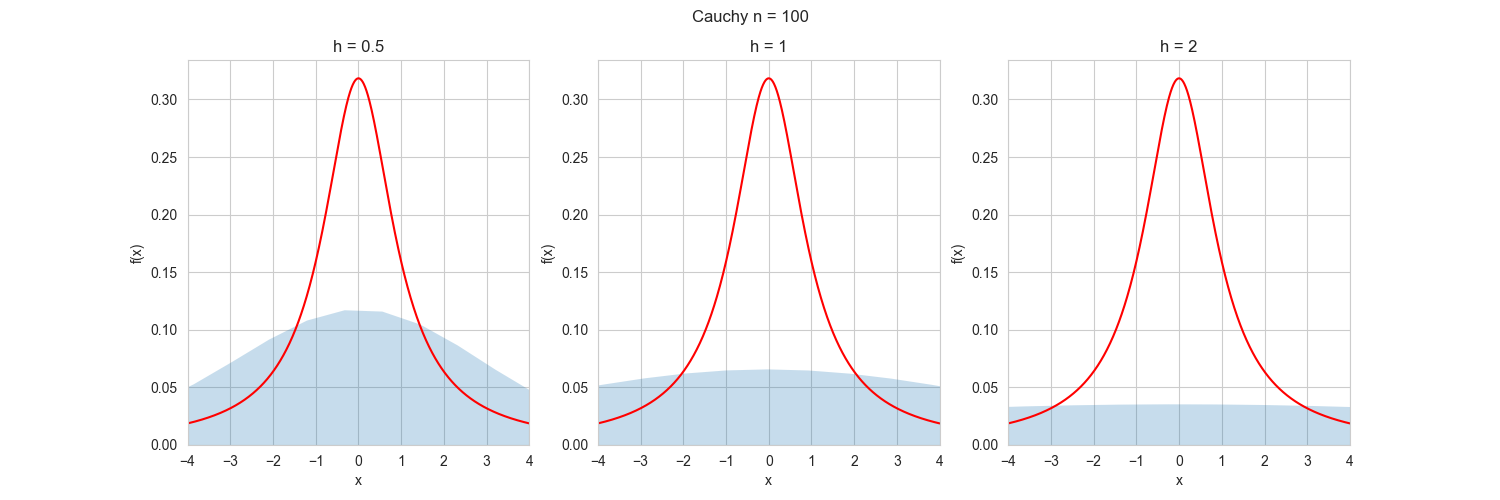
\includegraphics[scale=0.5]{figures/CauchyNuclear100.png}
        \caption{Распределение Коши, n = 100}
        \label{fig:normal}
    \end{figure}
    
    \begin{figure}[H]
        \centering
        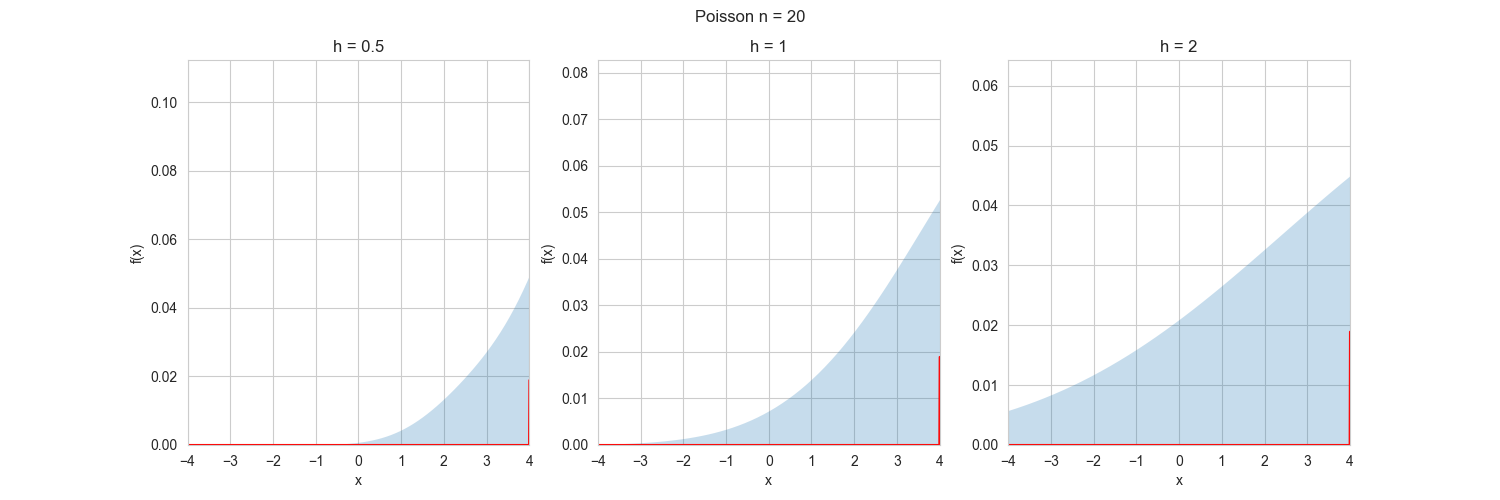
\includegraphics[scale=0.5]{figures/PoissonNuclear20.png}
        \caption{Распределение Пуассона, n = 20}
        \label{fig:normal}
    \end{figure}
    
    \begin{figure}[H]
        \centering
        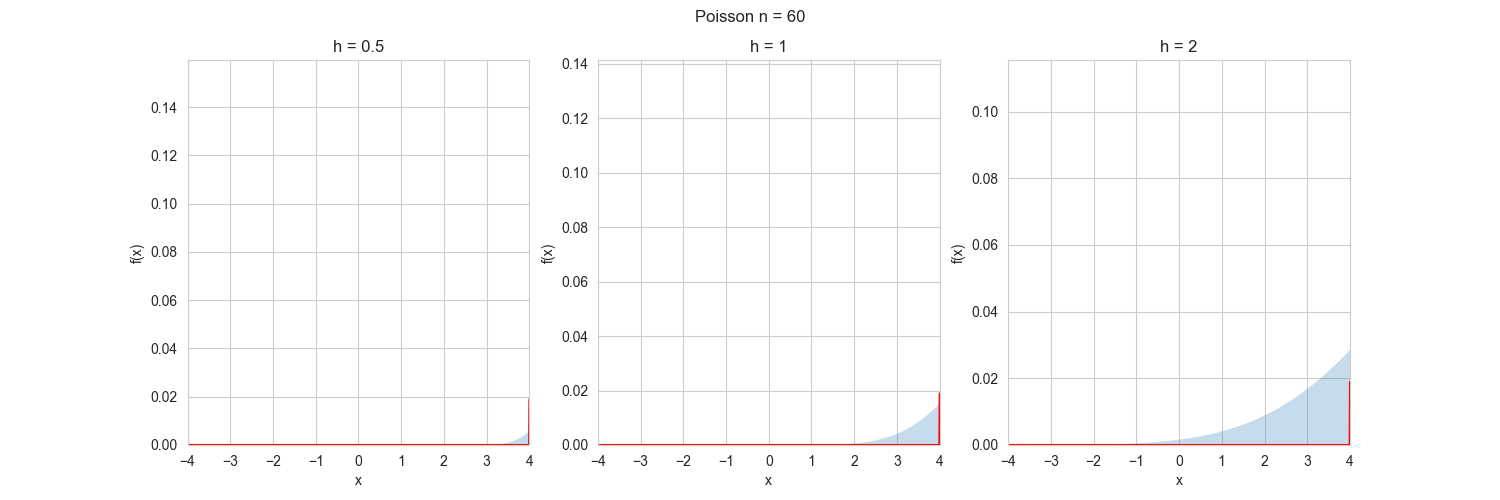
\includegraphics[scale=0.5]{figures/PoissonNuclear60.png}
        \caption{Распределение Пуассона, n = 60}
        \label{fig:normal}
    \end{figure}
    
    \begin{figure}[H]
        \centering
        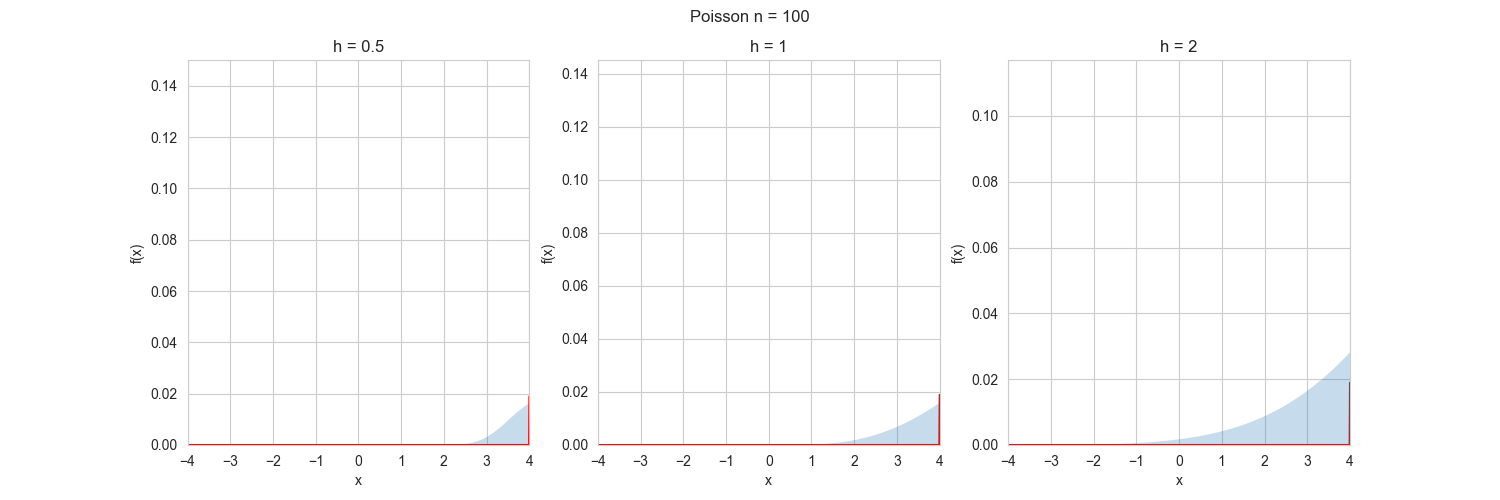
\includegraphics[scale=0.5]{figures/PoissonNuclear100.png}
        \caption{Распределение Пуассона, n = 100}
        \label{fig:normal}
    \end{figure}
    
    \begin{figure}[H]
        \centering
        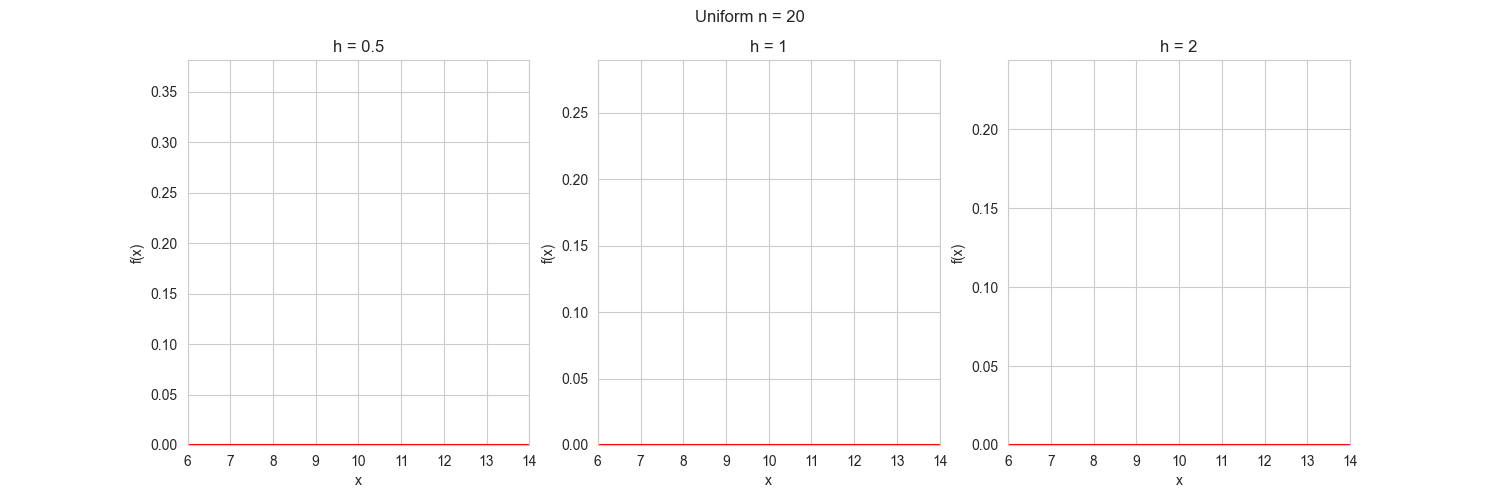
\includegraphics[scale=0.5]{figures/UniformNuclear20.png}
        \caption{Равномерное распределение, n = 20}
        \label{fig:normal}
    \end{figure}
    
    \begin{figure}[H]
        \centering
        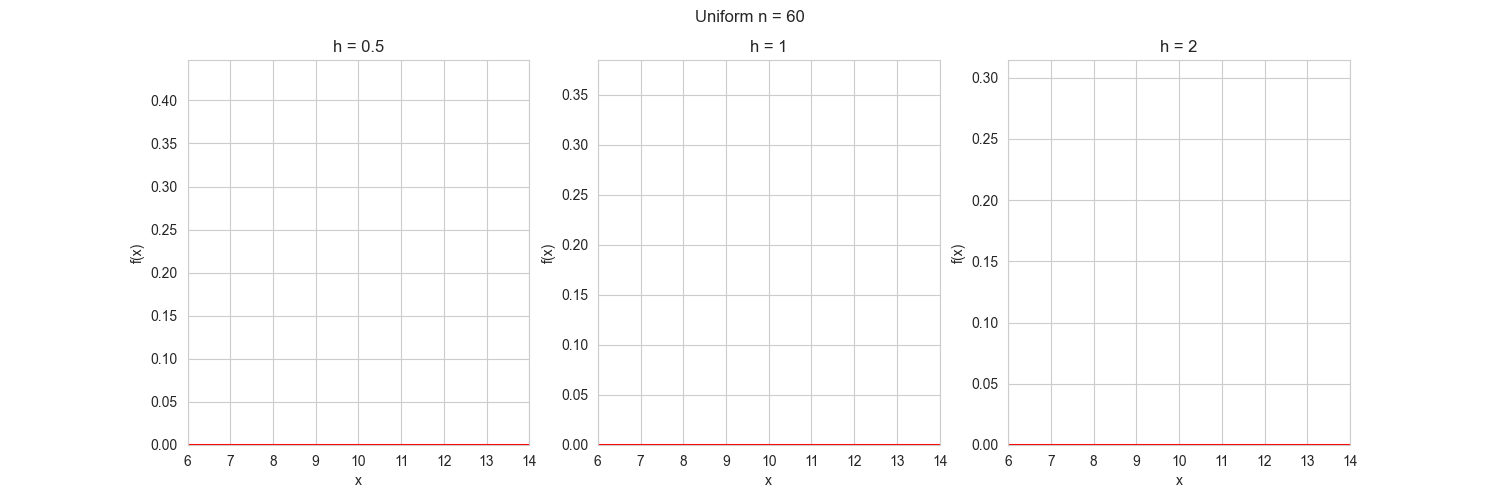
\includegraphics[scale=0.5]{figures/UniformNuclear60.png}
        \caption{Равномерное распределение, n = 60}
        \label{fig:normal}
    \end{figure}
    
    \begin{figure}[H]
        \centering
        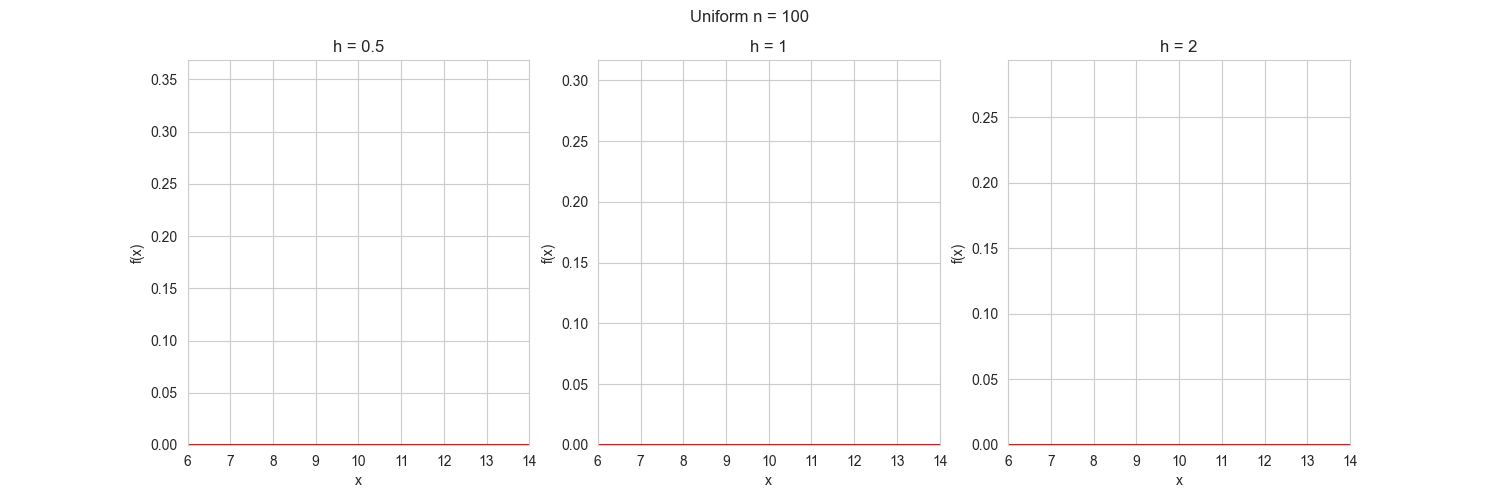
\includegraphics[scale=0.5]{figures/UniformNuclear100.png}
        \caption{Равномерное распределение, n = 100}
        \label{fig:normal}
    \end{figure}
\end{document}